\documentclass[a4paper]{article}
\usepackage{tikz}
\usepackage{amsmath}
\title{Acrobot}
\begin{document}
\maketitle
\begin{figure}[h]
\centering
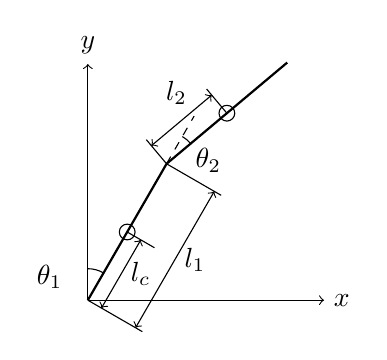
\begin{tikzpicture}
\draw[->] (0,0) -- (3,0) node[anchor=west] {$x$};
\draw[->] (0,0) -- (0,3) node[anchor=south] {$y$};

\draw (0,.4) arc(90:60:.4);
\draw (-.2,.3) node[anchor=east] {$\theta_1$};
\draw [thick] (0,0) -- (60:2);
\draw (60:1.0) circle(.1);
\draw (0,0) -- (-30:.8);
\draw [<->] (-30:.2) -- +(60:1.0);
\draw (-30:.2) +(60:.5) node[anchor=west] {$l_c$};
\draw [<->] (-30:.7) -- +(60:2.0);
\draw (-30:.7) +(60:1.0) node[anchor=west] {$l_1$};
\draw (60:1.0) -- +(-30:.4);
\draw (60:2.0) -- +(-30:.8);
\draw[dashed] (60:2) -- +(60:.7);
\draw (60:2.4) arc(60:40:.4);
\draw (60:2.0) +(10:.25) node[anchor=west] {$\theta_2$};
\draw [thick] (60:2) -- +(40:2);
\draw (60:2) -- +(130:.4);
\draw (60:2) ++(40:1) -- +(130:.4);
\draw [<->] (60:2) ++(130:.3) -- +(40:1);
\draw (60:2) ++(130:.4) ++(40:.5) node[anchor=south] {$l_2$};
\draw (60:2) +(40:1) circle(.1);
\end{tikzpicture}
\end{figure}

Position
\begin{eqnarray*}
x_1 &=& l_c \sin(\theta_1)\\
y_1 &=& l_c \cos(\theta_1)\\
\end{eqnarray*}
\begin{eqnarray*}
x_2 &=& l_1 \sin(\theta_1) + l_2 \sin(\theta_1 + \theta_2)\\
y_2 &=& l_1 \cos(\theta_1) + l_2 \cos(\theta_1 + \theta_2)
\end{eqnarray*}

Kinetic energy
\begin{eqnarray*}
T &=&\frac{1}{2} m_1 l_c^2 \dot{\theta}_1^2 + \frac{1}{2} m_2 l_1^2 \dot{\theta}_1^2
+ \frac{1}{2} m_2 l_2^2 (\dot{\theta}_1 + \dot{\theta_2})^2\\
&&+ m_2 l_1 l_2 \dot{\theta}_1(\dot{\theta}_1 + \dot{\theta}_2)
\left(\sin(\theta_1)\sin(\theta_1+\theta_2) + \cos(\theta_1)\cos(\theta_1+\theta_2)\right)\\
&=& \frac{1}{2} m_1 l_c^2 \dot{\theta}_1^2 + \frac{1}{2} m_2 l_1^2 \dot{\theta}_1^2
+ \frac{1}{2} m_2 l_2^2 (\dot{\theta}_1 + \dot{\theta_2})^2
+ m_2 l_1 l_2 \dot{\theta}_1(\dot{\theta}_1 + \dot{\theta}_2) \cos(\theta_2)\\
&=& \frac{1}{2} (m_1 l_c^2 + m_2 l_1^2 + m_2 l_2^2 + 2 m_2 l_1 l_2 \cos{\theta_2}) \dot{\theta}_1^2
+ m_2 (l_2^2 + l_1 l_2 \cos{\theta_2}) \dot{\theta}_1 \dot{\theta}_2
+ \frac{1}{2} m_2 l_2^2 \dot{\theta}_2^2\\
&=& \frac{1}{2}
\begin{pmatrix} \dot{\theta}_1 & \dot{\theta}_2 \end{pmatrix}\
\begin{pmatrix} m_1 l_c^2 + m_2 l_1^2 + m_2 l_2^2 + 2 m_2 l_1 l_2 \cos{\theta_2} &
    m_2 (l_2^2 + l_1 l_2 \cos{\theta_2})\\
    m_2 (l_2^2 + l_1 l_2 \cos{\theta_2}) &
    m_2 l_2^2 \end{pmatrix}
\begin{pmatrix} \dot{\theta}_1\\ \dot{\theta}_2 \end{pmatrix}
\end{eqnarray*}

Potential energy
\begin{eqnarray*}
V &=& m_1 g y_1 + m_2 g y_2\\
  &=& (m_1 l_c + m_2 l_1) g \cos{\theta_1} + m_2 l_2 g \cos(\theta_1 + \theta_2)
\end{eqnarray*}
\end{document}
